\section*{Experiments}
In this section, we briefly present our experiments on some of the 
algorithms presented at the previous sections. Two sets of experiments are presented.

The first tests are on powers
of random gaussian matrices of different sizes. The goal of this set of numerics
is to check the performance of the algorithms and make sure they are working
as expected. We also analyze the sharpness of the bounds dictated by the theory.
In particular, the bound on the expectation of the error given
by \ref{thm:avg-frob-error-gauss} and
the error estimation procedure which was motivated by 
Lemma \ref{thm:aposteriori}.

The second set of experiments is ...

\subsection{Details of the implementation}
The experiments have been performed in \verb|Matlab|. The reproducible
source code can be found at the following 
\href{https://github.com/alexnowakvila/ProbAlgosProj}{Github repository}
together with the \LaTeX  of the report.
\subsection{Gaussian Matrices}
In this set of experiments, we test and analyze the performance of the 
Algorithms \ref{alg:randomized-range-finder}, 
\ref{alg:adaptive-randomized-range-finder},
\ref{alg:randomized-power-iteration}
and \ref{alg:fast-randomized-range-finder}.

The experiments are performed on powers of gaussian random
matrices of the form:

\begin{equation}\label{eq:gaussian-matrices}
\mtx{A} = \frac{1}{\sqrt{m}+\sqrt{n}}\mtx{G}, \hspace{0.5cm}
 G_{ij}\sim N(0,1)
\end{equation}
The normalization in \ref{eq:gaussian-matrices} is to make sure that the norm
of $\mtx{A}$ is around 1 with high probability
\footnote{This is a direct consequence of Sudakov-Fernique's inequality that
compares the supremum of two gaussian processes when one is dominated
by the other. More precisely, you have the bound on the expectation
of the norm $\Expect\|\mtx{G}\|\leq\sqrt{m}+\sqrt{n}$
and also an accompanying tail bound 
$\Prob{\|\mtx{G}\| \geq \sqrt{m} + \sqrt{n} + t}\leq 2\exp(-ct^2)$.
Using Gordon's inequality (generalization of Sudakov Fernique's), you can
also prove lower bounds on the smallest singular value
$\Expect\|\mtx{G}^\dagger\|\geq \sqrt{m} - \sqrt{n}$ and
$\Prob{\|\mtx{G}\|\leq \sqrt{m}-\sqrt{n}-t}\leq 2\exp(-ct^2)$.
These results on concentration of measure have been studied at the Theory
Reading Group following the book on High Dimensional Probability
from R.Vershynin which I highly recommend 
\cite{vershynin2016high}.}.

\subsubsection{Experiments on Randomized Range Finder 
\ref{alg:randomized-range-finder}}

\begin{figure}[ht]
\begin{center}
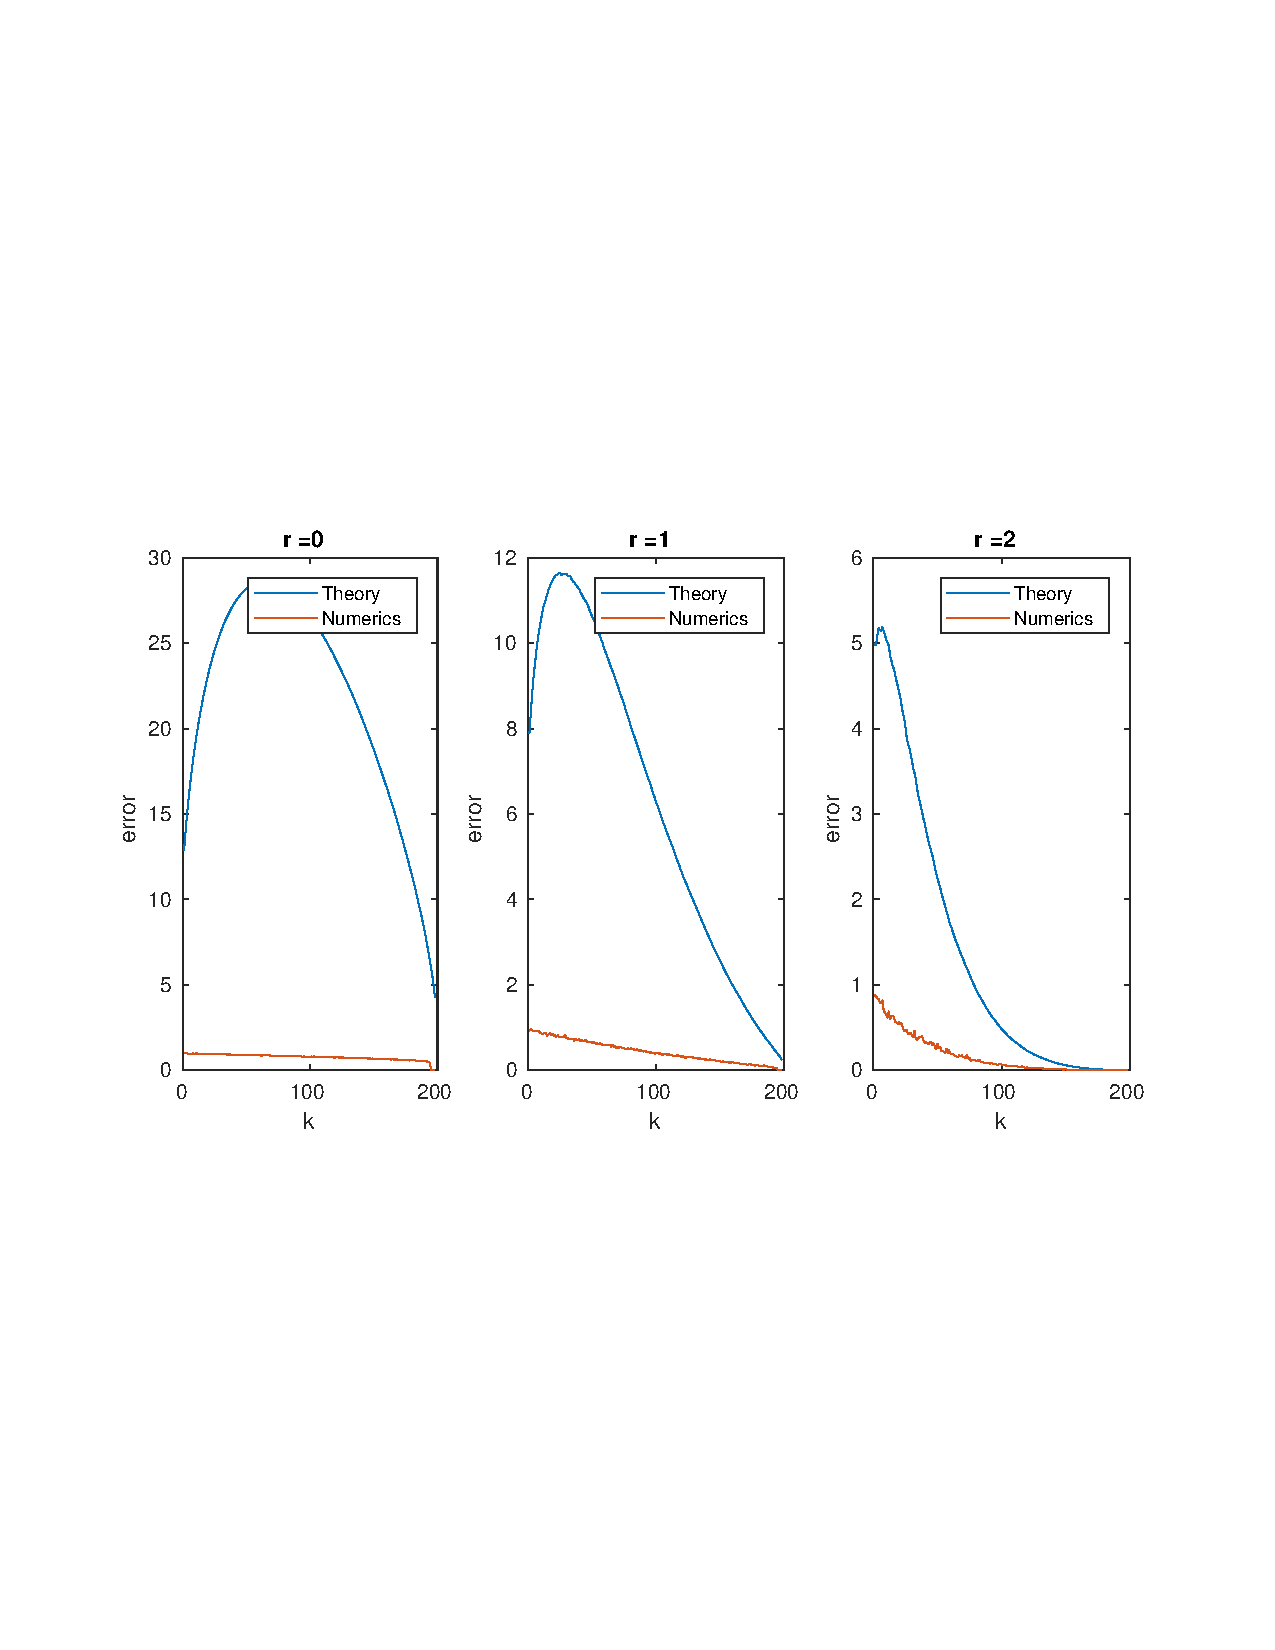
\includegraphics[width=\textwidth]{figures/1-4.pdf}
\end{center}
\caption{bla}
\end{figure}

\subsubsection{Experiments on Randomized Power Iteration 
\ref{alg:randomized-power-iteration}}

\begin{figure}[ht]
\begin{center}
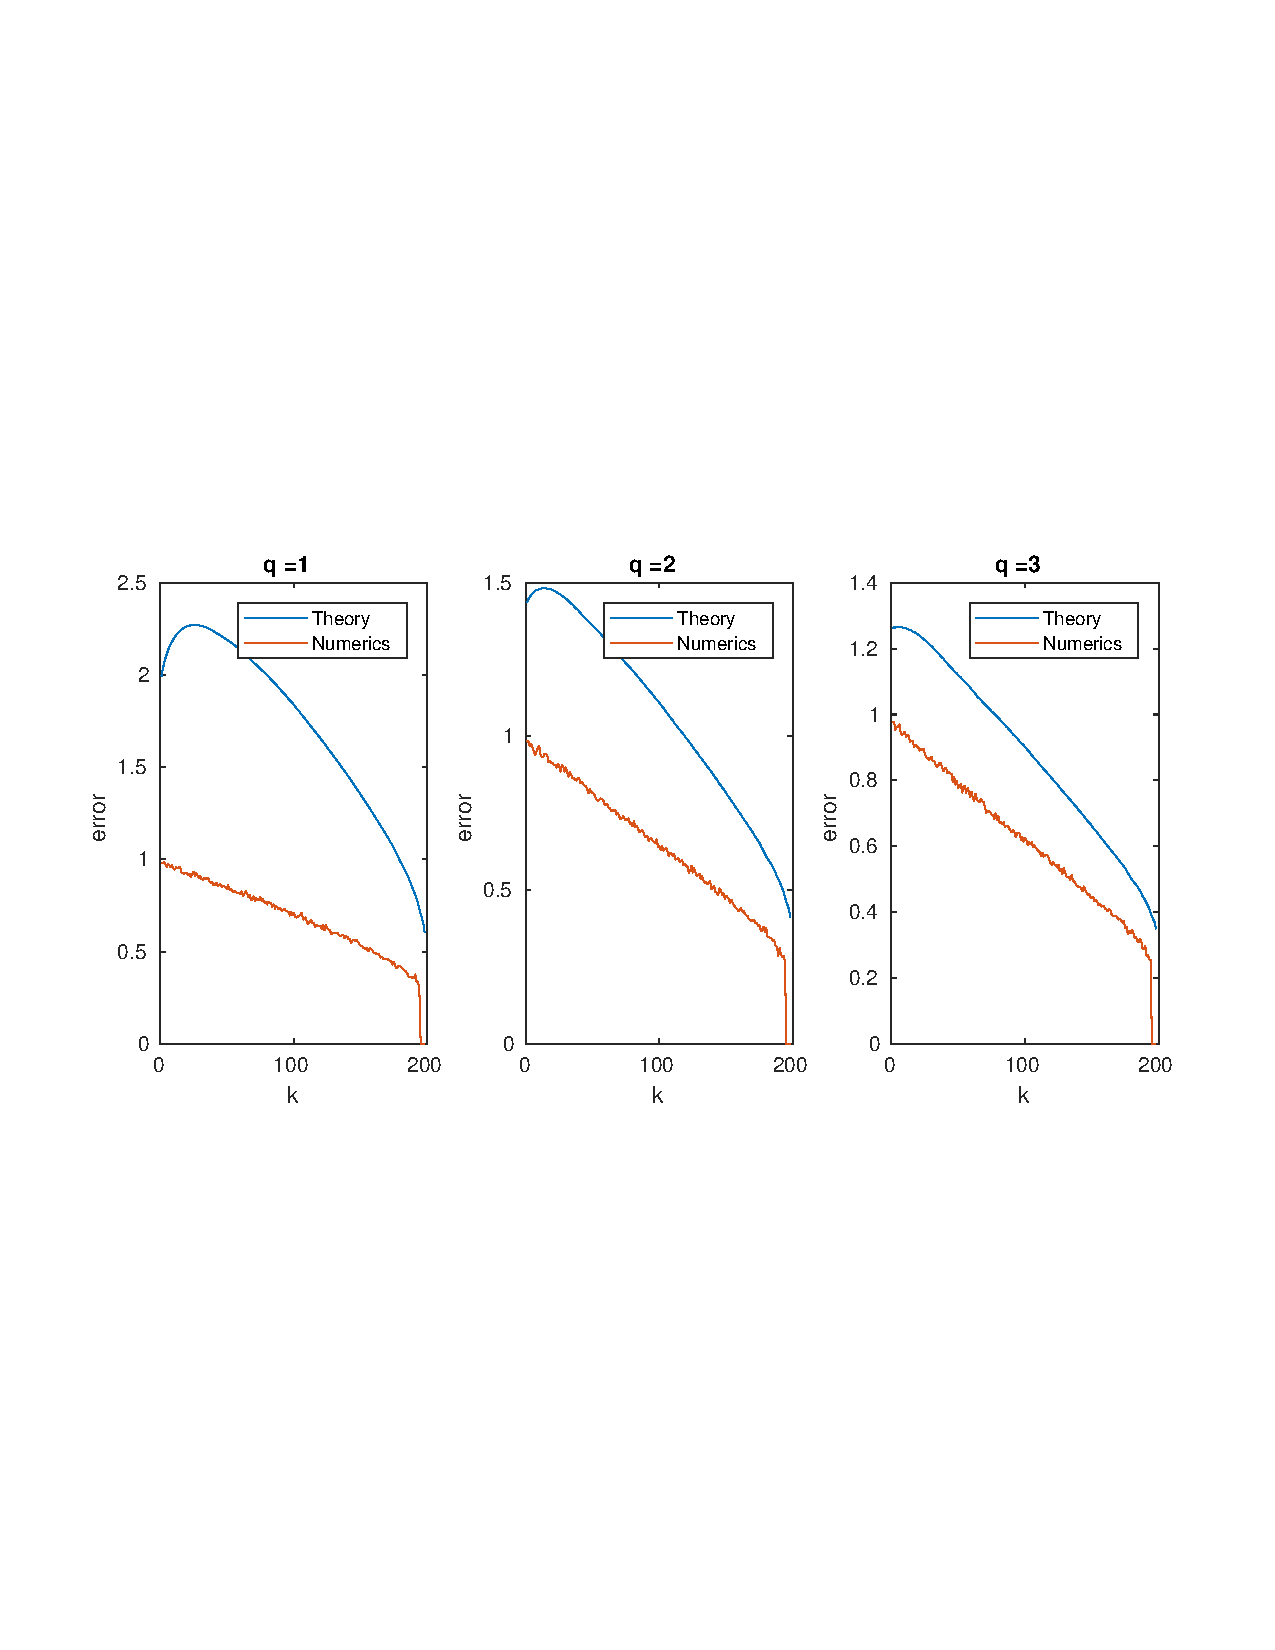
\includegraphics[width=\textwidth]{figures/1-5.pdf}
\end{center}
\caption{bla}
\end{figure}

\subsubsection{Experiments on Adaptive Randomized Range Finder
\ref{alg:adaptive-randomized-range-finder}}

\subsubsection{Experiments on Fast Randomized Range Finder
\ref{alg:fast-randomized-range-finder}}
\label{sec:gaussian-matrices}
\subsection{Real Dataset}